% !TeX root = statnicaEKT.tex
\part{BPC-MVA - Měření v elektrotechnice}
{\huge Otázky:}
\newline
\begin{enumerate}
	\item Otázka - Nejistota přímého a nepřímého měření; přístrojová nejistota; odchylka měření a metody. 
	\item Otázka - Měření aktivních elektrických veličin; stejnosměrné a časově proměnné napětí a proud, výkon, kmitočet, fázový posun.
	\item Otázka - Měření pasivních elektrických veličin; odpor, impedance. 
\end{enumerate}
\newpage
\chapter{Nejistoty, odchylky a metody měření}
\label{ch:nejistoty}

\noindent\textit{Definice přímého a nepřímého měření, klasifikace chyb (odchylek) měření, metody měření (substituční, kompenzační, diferenciální, můstkové), třída přesnosti analogových přístrojů, chyby digitálních přístrojů, stanovení nejistot typu A a typu B, kombinovaná a rozšířená nejistota, zápis výsledku.}

\section{Úvod a metrologické etalony}
Měření je proces kvantitativního porovnávání měřené veličiny s jednotkou.
\begin{itemize}
    \item \textbf{Přímé měření:} Hodnotu veličiny odečteme přímo na měřicím přístroji (např. měření napětí multimetrem).
    \item \textbf{Nepřímé měření:} Hodnotu určíme výpočtem z jiných přímo naměřených veličin (např. stanovení výkonu $P = U \cdot I$).
\end{itemize}

Návaznost měřidel je zajištěna hierarchickým systémem etalonů spravovaným organizacemi BIPM (mezinárodní úroveň), ÚNMZ a ČMI (státní úroveň v ČR).

\subsection{Kvantové etalony}
Moderní metrologie se opírá o fundamentální fyzikální konstanty.

\noindent\textbf{Josephsonův napěťový etalon:} Supravodivý Josephsonův přechod ozařovaný kmitočtem $f_0 \approx 10\text{ GHz}$ generuje diskrétní kroky napětí:
\[ U_n = n \frac{f_0}{K_J} \]
kde $K_J = \frac{2e}{h} \approx 483\,597{,}898\text{ GHz/V}$ je Josephsonova konstanta.

\noindent\textbf{Kvantový etalon odporu (Klitzingův):} Využívá kvantový Hallův jev ve dvojrozměrném elektronovém plynu za nízkých teplot a silných magnetických polí:
\[ R_K = \frac{h}{e^2} \approx 25\,812{,}807\ \Omega \]
kde $R_K$ je von Klitzingova konstanta.

\section{Odchylky (chyby) měření}
Odchylka měření vyjadřuje rozdíl mezi naměřenou hodnotou $X_M$ a skutečnou (či konvenčně pravou) hodnotou $X_P$.

\noindent\textbf{Absolutní odchylka} má rozměr měřené veličiny:
\[ \Delta = X_M - X_P \]
\textbf{Relativní odchylka} je bezrozměrná veličina vyjadřující poměrnou velikost chyby k pravé hodnotě:
\[ \delta = \frac{\Delta}{X_P} \cdot 100\ [\%] \approx \frac{\Delta}{X_M} \cdot 100\ [\%] \]

\subsection{Klasifikace chyb podle původu a vlastností}
\begin{itemize}
    \item \textbf{Systematické odchylky ($\Delta_{SYST}$):} Mění se předvídatelně nebo zůstávají konstantní. Jsou způsobeny nedokonalostí přístrojů, vlivem prostředí či metodou. Lze je matematicky korigovat (přičtením korekce $C = -\Delta_{max}$).
    \item \textbf{Náhodné odchylky:} Kolísají nepravidelně vlivem mnoha neznámých a nestálých příčin. Mají symetrické rozdělení pravděpodobnosti (Gaussovo/normální rozdělení) a nelze je individuálně korigovat, pouze statisticky vyhodnotit.
    \item \textbf{Hrubé odchylky (omyly):} Způsobené nepozorností obsluhy, poruchou. Měření zatížené hrubou chybou se musí z řady vyloučit.
\end{itemize}

\begin{figure}[h]
\centering
\begin{tikzpicture}[>=stealth, scale=1.05]
  \draw[->] (-3.8,0) -- (3.8,0) node[right,font=\small] {Odchylka $\Delta$};
  \draw[->] (0,-0.15) -- (0,1.95) node[above,font=\small] {$p(\Delta)$};
  \fill[secondary!15] (-2,0) -- plot[domain=-2:2,samples=50] (\x,{1.55*exp(-\x*\x/2)}) -- (2,0) -- cycle;
  \fill[secondary!40] (-1,0) -- plot[domain=-1:1,samples=30] (\x,{1.55*exp(-\x*\x/2)}) -- (1,0) -- cycle;
  \draw[thick,primary,domain=-3.5:3.5,samples=80] plot (\x,{1.55*exp(-\x*\x/2)});
  \foreach \xval/\xlbl in {-3/$-3\sigma$,-2/$-2\sigma$,-1/$-\sigma$,1/$+\sigma$,2/$+2\sigma$,3/$+3\sigma$} {
    \draw (\xval,0.06) -- (\xval,-0.06) node[below,font=\scriptsize] {\xlbl};
  }
  \node[below,font=\scriptsize] at (0,-0.06) {$\mu$};
  \node[font=\scriptsize,primary!80!black] at (0,0.52) {68{,}3\,\%};
  \draw[<->,primary!70!black] (-1,-0.32) -- (1,-0.32) node[midway,below,font=\scriptsize] {$\pm\sigma$};
  \draw[<->,secondary!70!black] (-2,-0.52) -- (2,-0.52) node[midway,below,font=\scriptsize] {$\pm 2\sigma$: 95{,}4\,\%};
\end{tikzpicture}
\caption{Gaussovo (normální) rozdělení náhodných chyb kolem střední hodnoty $\mu$. Interval $\pm\sigma$ pokrývá 68{,}3\,\% výsledků, interval $\pm 2\sigma$ pokrývá 95{,}4\,\%.}
\label{fig:gauss}
\end{figure}

\section{Základní metody měření}
K eliminaci systematických chyb a zvýšení přesnosti se používají různé metody:
\begin{itemize}
    \item \textbf{Výchylková metoda:} Hodnota se určí přímo z výchylky ukazatele (rychlé, méně přesné).
    \item \textbf{Substituční (nahrazovací) metoda:} Neznámá veličina se nahradí známým nastavitelným etalonem stejného druhu tak, aby se indikovaná výchylka nezměnila. Odstraňuje chybu vlastního měřicího přístroje.
    \item \textbf{Kompenzační metoda:} Porovnává měřenou veličinu s etalonem tak, aby ve stavu rovnováhy obvodem netekl proud (např. napěťový kompenzátor). Vstupní odpor je v rovnováze teoreticky nekonečný.
    \item \textbf{Diferenciální (rozdílová) metoda:} Měří se pouze rozdíl mezi neznámou veličinou a blízkým etalonem. Umožňuje použít citlivý přístroj na malém rozsahu.
    \item \textbf{Můstková metoda:} Využívá vyvážení nebo výchylku můstkového zapojení (kombinace kompenzační a rozdílové metody).
\end{itemize}

\section{Odchylky a nejistoty měřicích přístrojů}

\subsection{Analogové přístroje a třída přesnosti}
Třída přesnosti $TP$ udává maximální dovolenou absolutní odchylku jako procento z plného rozsahu (měřicího rozsahu) $M$:
\[ \Delta_{max} = \pm \frac{TP \cdot M}{100} \]
Z toho vyplývá, že relativní chyba přístroje strmě roste při měření na začátku stupnice ($\delta \propto \Delta_{max}/X_M$). Proto volíme rozsah tak, aby výchylka byla v poslední třetině stupnice.

\subsection{Číslicové (digitální) přístroje}
Chyba se u číslicových multimetrů skládá ze dvou složek: chyby zesílení/převodu (procento z měřené hodnoty $rdg$) a chyby linearity/posunu (procento z rozsahu $range$ nebo počet jednotek nejnižšího řádu $digits$):
\begin{align*}
\Delta_{max} &= \pm (a\% \cdot X_M + b\% \cdot M) \\
\text{nebo} \quad \Delta_{max} &= \pm (a\% \cdot X_M + d \cdot \text{digit})
\end{align*}

\section{Vyhodnocování nejistot měření}
Nejistota měření je parametr přidružený k výsledku měření, který charakterizuje rozptyl hodnot.

\subsection{Nejistota typu A (\texorpdfstring{$u_{AX}$}{u_AX})}
Stanovuje se statistickým zpracováním řady $m$ opakovaných nezávislých měření téže veličiny za stejných podmínek. Standardní nejistota typu A:
\[ u_{AX} = k_s \cdot \sqrt{\frac{1}{m(m-1)} \sum_{k=1}^{m} (X_k - \overline{X})^2} \]
kde $\overline{X} = \frac{1}{m}\sum_{k=1}^m X_k$ je aritmetický průměr, $m$ je počet měření a $k_s$ je korekční součinitel (pro $m \ge 10$ se uvažuje $k_s = 1$).

\subsection{Nejistota typu B (\texorpdfstring{$u_B$}{u_B})}
Určuje se nestatistickými metodami na základě dostupných informací (specifikace výrobce, kalibrační listy). Vychází se z maximální dovolené chyby $\Delta_{max}$ a předpokládaného rovnoměrného (pravoúhlého) rozdělení:
\[ u_B = \frac{\Delta_{max}}{\sqrt{3}} \approx 0{,}58 \cdot \Delta_{max} \]
Při více nezávislých zdrojích nejistot typu B: $u_B = \sqrt{\sum_{i} u_{Bi}^2}$

\subsection{Kombinovaná a rozšířená nejistota}
Pro přímé měření se sloučí nejistoty typu A a B kvadraticky:
\[ u_c = \sqrt{u_A^2 + u_B^2} \]
Pro nepřímé měření $y = f(x_1, x_2, \dots, x_m)$ platí zákon šíření nejistot:
\[ u_c(y) = \sqrt{\sum_{i=1}^m \left(\frac{\partial f}{\partial x_i}\right)^2 u_c^2(x_i)} \]
Rozšířená nejistota určuje interval spolehlivosti:
\[ U = k \cdot u_c \]
kde $k$ je koeficient rozšíření (standardně $k=2$ odpovídá pravděpodobnosti pokrytí $\approx 95\%$).

\subsection{Zápis výsledku měření}
Výsledek se zaokrouhluje tak, aby nejistota měla maximálně dvě platné číslice. Hodnota se zaokrouhlí na stejné desetinné místo jako rozšířená nejistota:
\[ X = (\bar{X} \pm U)\ \text{[jednotka]} \quad \text{pro } k=2 \]


\chapter{Měření aktivních elektrických veličin}
\label{ch:aktivni_veliciny}

\noindent\textit{Princip a vlastnosti elektromechanických ústrojí, analogové aktivní a pasivní převodníky (usměrňovače, TRMS převodníky, Rogowskiho cívka, měřicí transformátory), řetězec digitalizace (Shannon-Nyquist teorém, aliasing, AD převodníky), digitální osciloskopy, spektrální analýza, měření proudu, napětí, výkonu (Aronovo zapojení v 3f), měření frekvence a fázového posuvu.}

\section{Elektromechanická měřicí ústrojí}
Využívají silové účinky proudů a polí k otočení ručky. Pohybový moment $M_P$ působí proti direktivnímu (vratnému) momentu pružiny $M_D = k_D \cdot \alpha$. V rovnováze: $M_P = M_D$.

\begin{table}[h]
\centering
\small
\caption{Přehled základních elektromechanických ústrojí}
\vspace{0.2cm}
\begin{tabular}{p{2.8cm}p{2.4cm}cp{2.5cm}p{3.4cm}}
\toprule
\textbf{Ústrojí} & \textbf{Značka} & \textbf{Výchylka} $\alpha$ & \textbf{Druh proudu} & \textbf{Použití} \\
\midrule
Magnetoelektrické & Deprez & $\propto I$ & DC (střední hodnota) & Ampérmetry, voltmetry \\
Feromagnetické & Měkké železo & $\propto I^2$ & AC i DC (efektivní) & Síťové ampérmetry, voltmetry \\
Elektrodynamické & Bezželezné cívky & $\propto I_1 I_2 \cos \varphi$ & AC i DC (činný výkon) & Wattmetry \\
Indukční & Vířivé proudy & $\propto I_1 I_2 \sin \psi$ & Pouze AC & Elektroměry (starší) \\
Elektrostatické & Náboj & $\propto U^2$ & AC i DC (efektivní) & Vysoké napětí \\
\bottomrule
\end{tabular}
\end{table}

\begin{itemize}
    \item \textbf{Magnetoelektrické (Deprezské):} Otočná cívka v permanentním magnetickém poli. Vysoká citlivost, lineární stupnice. Reaguje pouze na DC složku (střední hodnotu). U AC signálu střední hodnota zaniká a setrvačnost ručky zabrání pohybu. S usměrňovačem měří střední absolutní hodnotu AC signálu.
    \item \textbf{Feromagnetické:} Pevná cívka vtahující nebo odpuzující jádro z magneticky měkkého materiálu. Robustní, levné, kvadratická stupnice. Ukazuje skutečnou efektivní hodnotu (TRMS) i u zkreslených střídavých průběhů.
    \item \textbf{Elektrodynamické (wattmetr):} Silové působení dvou cívek -- pevná \textbf{proudová cívka} zapojena v sérii se zátěží ($i_1 = i_Z$), otočná \textbf{napěťová cívka} zapojena paralelně přes předřadný odpor $R_{WU}$ ($i_2 = u/R_{WU}$). Střední pohybový moment je:
    \[ M_P = k_P \cdot I_1 \cdot I_2 \cdot \cos\varphi = k_P \cdot \frac{U \cdot I \cdot \cos\varphi}{R_{WU}} = k_P \cdot \frac{P}{R_{WU}} \]
    Výchylka je přímo úměrná činnému výkonu $P$, nezávisle na tvaru průběhu.
\end{itemize}

\begin{figure}[H]
\centering
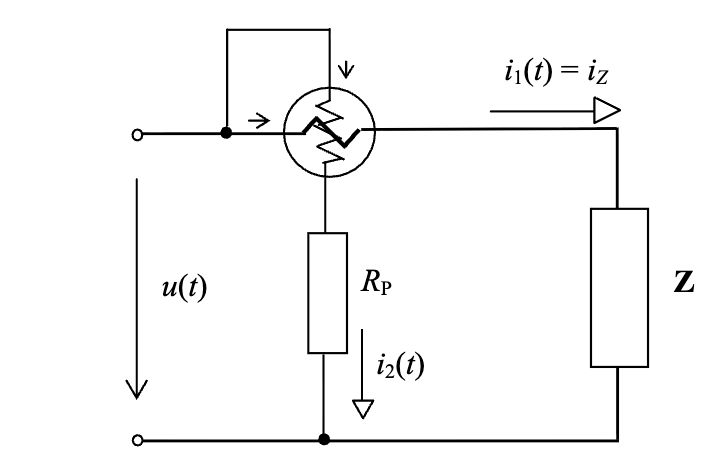
\includegraphics[width=0.70\textwidth]{Obrazky/MVA/wattmetr}
\caption{Schéma elektrodynamického wattmetru. Proudová cívka (série se zátěží) a napěťová cívka (paralelně přes $R_{WU}$). Výchylka $\propto P = U I \cos\varphi$.}
\label{fig:wattmetr}
\end{figure}

\section{Analogové měřicí převodníky a transformátory}

\subsection{Usměrňovače s operačním zesilovačem}
Pasivní diodové usměrňovače mají prahové napětí $\approx 0{,}7\,\text{V}$, což znemožňuje přesné usměrňování malých napětí. Operační zesilovač (OZ) se zpětnou vazbou přes diodu tuto chybu kompenzuje -- dioda je umístěna v uzavřené zpětnovazební smyčce, takže výstup OZ automaticky dodá napětí potřebné k jejímu otevření.

\begin{figure}[H]
\centering
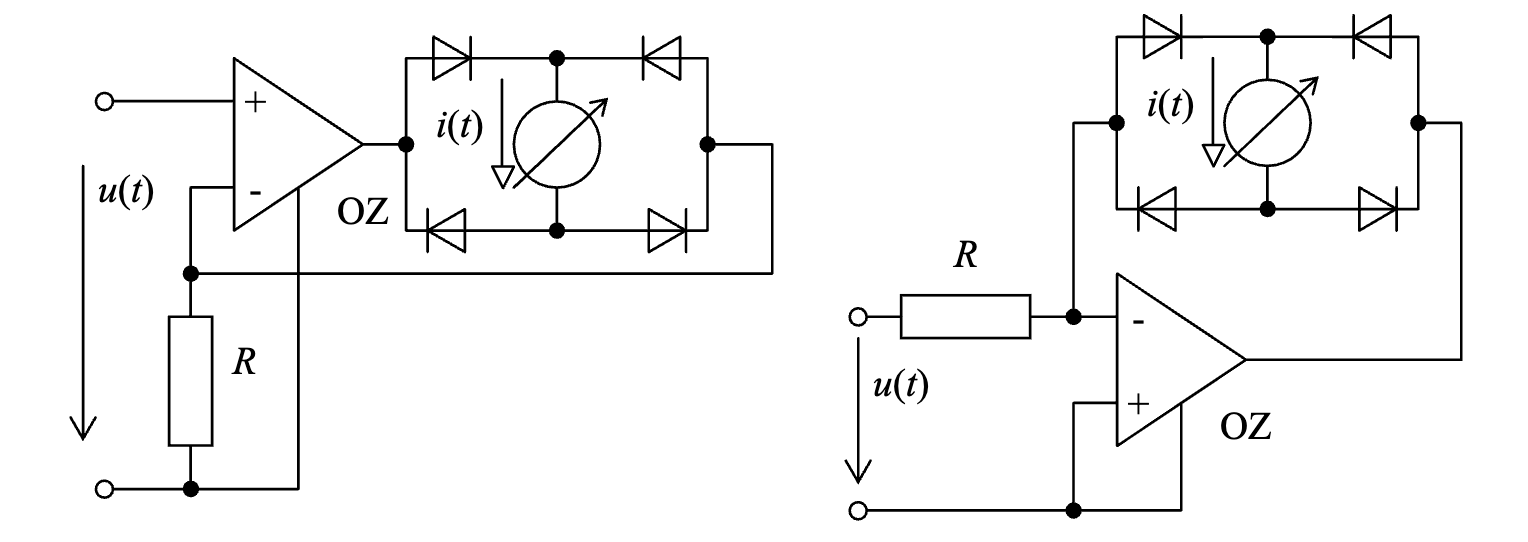
\includegraphics[width=0.75\textwidth]{Obrazky/MVA/dvucestnyusmernovac}
\caption{Příklady zapojení aktivního dvoucestného usměrňovače s OZ (obr.~4.14). Diody jsou ve zpětnovazební větvi; usměrněný proud v měřidle je přímo úměrný vstupnímu napětí nezávisle na prahu diod.}
\label{fig:usm_oz}
\end{figure}

Pasivní usměrňovač spolu s magnetoelektrickým ústrojím reaguje na \textbf{střední absolutní hodnotu} $U_{sa} = \frac{1}{T}\int_0^T |u(t)|\,\mathrm{d}t$. Protože jsou přístroje cejchovány pro sinusový průběh, zavádějí se:

\noindent\textbf{Činitel tvaru a činitel výkyvu:}
\[ k_t = \frac{U}{U_{sa}} \quad \text{(činitel tvaru)}, \qquad k_v = \frac{\hat{U}}{U} \quad \text{(činitel výkyvu)} \]
Pro sinusový průběh: $k_{t,\sin} = \dfrac{\pi}{2\sqrt{2}} \approx 1{,}111$, \quad $k_{v,\sin} = \sqrt{2} \approx 1{,}414$.\\
Pro obdélníkový průběh: $k_t = 1{,}000$, \quad $k_v = 1{,}000$.

\noindent Přístroj zobrazuje $k_{t,\sin}\cdot U_{sa}$. Při měření \textbf{nesinusového průběhu} vzniká \textit{chyba tvaru}: $\delta = (k_t/k_{t,\sin} - 1)\cdot 100\,\%$. Pro neharmonické signály je nutný TRMS převodník.

\subsection{Převodníky TRMS}
Měří skutečnou efektivní hodnotu (True RMS) podle definice:
\[ U_{RMS} = \sqrt{\frac{1}{T}\int_0^T u^2(t)\,\mathrm{d}t} \]

\begin{figure}[H]
\centering
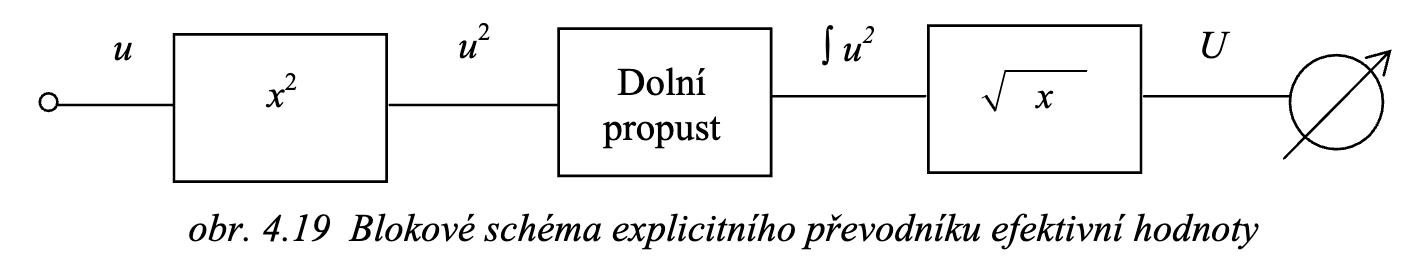
\includegraphics[width=0.72\textwidth]{Obrazky/MVA/TRMS}
\caption{Blokové schéma explicitního TRMS převodníku (obr.~4.19). Vstup je umocněn (kvadrátor), zintegrován (průměr $\langle u^2 \rangle$) a odmocněn -- výsledek je $U_{RMS}$.}
\label{fig:trms}
\end{figure}

\begin{itemize}
    \item \textbf{Analogové výpočetní (explicitní):} Realizují operaci $\sqrt{\langle u^2 \rangle}$ bloky kvadrátor--integrátor--odmocnina (obr.~\ref{fig:trms}).
    \item \textbf{Termické (implicitní):} Vstupní signál ohřívá topný odporník; teplota (úměrná $u^2$) se snímá termočlánkem. Druhý termočlánek napájený ze stejnosměrného výstupu zajišťuje zpětnou vazbu. Frekvenčně nejnezávislejší -- vhodné až do MHz.
\end{itemize}

\subsection{Měřicí transformátory a Rogowskiho cívka}
Používají se k galvanickému oddělení a úpravě rozsahů u střídavých vysokých napětí a velkých proudů.
\begin{itemize}
    \item \textbf{Měřicí transformátor napětí (MTN):} Pracuje naprázdno (vysoká impedance sekundáru). Sekundár nesmí být zkratován -- hrozí přetížení proudem.
    \item \textbf{Měřicí transformátor proudu (MTP):} Pracuje nakrátko (nízká impedance sekundáru). \textbf{VAROVÁNÍ!} Sekundár nesmí být nikdy rozpojen pod proudem -- bez demagnetizačního pole se jádro přesytí a na sekundáru se indukují napětí v řádu kV.
    \item \textbf{Rogowskiho cívka:} Vzduchový toroid bez feromagnetického jádra obepínající vodič. Výstupní napětí: $u_{out}(t) = M \frac{di(t)}{dt}$. Pro rekonstrukci průběhu proudu je nutná integrace. Výhody: naprostá linearita, nemožnost přesycení, snadná instalace.
\end{itemize}

\section{Digitalizace a A/Č převodníky}
Převod spojitého signálu na diskrétní časové řady a digitální hodnoty.

\subsection{Shannon-Nyquistův teorém a Aliasing}
\noindent\textbf{Shannon-Nyquistův vzorkovací teorém:} Pro bezchybnou rekonstrukci musí být vzorkovací kmitočet $f_s$ alespoň dvakrát vyšší než maximální frekvenční složka signálu $f_{max}$:
\[ f_s > 2 \cdot f_{max} \]
Při nedodržení vzniká \textbf{aliasing} -- falešné nízkofrekvenční složky ve spektru. K jeho zamezení se před vzorkovač řadí analogový filtr typu dolní propust -- \textbf{antialiasingový filtr}.

\begin{figure}[h]
\centering
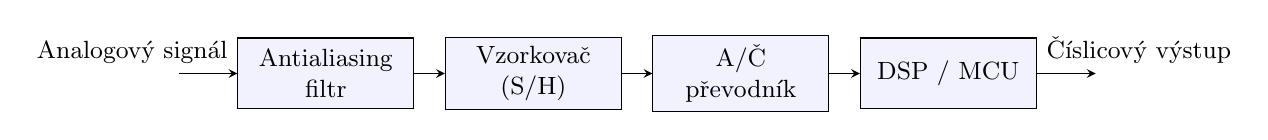
\begin{tikzpicture}[>=stealth, scale=0.85, block/.style={draw, fill=blue!5, rectangle, minimum height=0.9cm, minimum width=2.2cm, align=center, text width=2.0cm, font=\small}]
  \node [block] (aa) at (0,0) {Antialiasing filtr};
  \node [block] (sh) at (3.1,0) {Vzorkovač (S/H)};
  \node [block] (adc) at (6.2,0) {A/Č převodník};
  \node [block] (dsp) at (9.3,0) {DSP / MCU};

  \draw [->] (-2.2,0) -- (aa.west);
  \node[anchor=south east, font=\small] at (aa.west) {Analogový signál};
  \draw [->] (aa) -- (sh);
  \draw [->] (sh) -- (adc);
  \draw [->] (adc) -- (dsp);
  \draw [->] (dsp.east) -- (11.5,0);
  \node[anchor=south west, font=\small] at (dsp.east) {Číslicový výstup};
\end{tikzpicture}
\caption{Blokové schéma řetězce digitalizace signálu}
\label{fig:dig_chain}
\end{figure}

\subsection{Typy A/Č převodníků}
\begin{itemize}
    \item \textbf{Flash (komparační):} Nejrychlejší (GS/s), rozlišení obvykle 8 bitů. Obsahuje $2^N-1$ komparátorů. Používá se v osciloskopech.
    \item \textbf{SAR (s postupnou aproximací):} Využívá registr postupné aproximace a vnitřní D/A převodník k půlení intervalu. Vyžaduje $N$ taktů na jeden převod. Běžně 12--16 bitů, rychlosti MS/s. Běžné v mikrokontrolérech.
    \item \textbf{Integrační (dvojitá integrace):} Měřené napětí integruje po pevný čas, následně vybíjí referenčním napětím. Velmi pomalý, ale extrémně přesný s vysokou odolností proti síťovému rušení (50 Hz). Používá se v digitálních multimetrech.
    \item \textbf{Sigma-Delta ($\Sigma\Delta$):} Využívá vysoké převzorkování ($f_s \gg 2f_{max}$) a tvarování šumu (přesun šumu do vyšších kmitočtů). Velmi vysoké rozlišení (24 bitů) pro audio a přesná měření.
\end{itemize}

\section{Digitální osciloskopy a spektrální analyzátory}

\subsection{Struktura osciloskopu}
\begin{itemize}
    \item \textbf{Vertikální systém:} Zeslabovače, zesilovače, Flash ADC. Nastavuje vertikální citlivost (V/div) a šířku pásma.
    \item \textbf{Horizontální systém:} Časová základna (s/div), vzorkovací paměť.
    \item \textbf{Spouštění (Trigger):} Synchronizuje vzorkování s periodickým dějem (např. spouštění hranou, šířkou impulsu). Zajišťuje stabilní obraz na displeji.
    \item \textbf{Vliv sondy:} Pasivní sonda 10:1 zvětšuje vstupní odpor na $10\text{ M}\Omega$ a snižuje vstupní kapacitu (cca 10 pF). Trimrem na sondě se kompenzuje kapacitní dělič (frekvenční nezávislost) podle obdélníkového kalibračního signálu.
\end{itemize}

\subsection{Spektrální analyzátory}
\begin{itemize}
    \item \textbf{Superheterodynní (analogové):} Rozmítaný místní oscilátor směšuje vstupní signál s pilovým průběhem. Výsledný signál prochází úzkou pásmovou propustí na detektor. Široký frekvenční rozsah (desítky GHz).
    \item \textbf{FFT analyzátory (číslicové):} Spočítají spektrum z časového záznamu algoritmem rychlé Fourierovy transformace. Vhodné pro nízké frekvence a přechodové jevy.
\end{itemize}

\section{Měření napětí, proudu a výkonu}

\subsection{Měření napětí a proudu}

\textbf{Voltmetry} se připojují paralelně. Vstupní odpor $R_V$ musí být co největší. Rozšíření rozsahu: předřadný odpor $R_P = R_V(n-1)$, kde $n = U_{\text{nový}}/U_{\text{původní}}$.

\textbf{Kompenzační metoda:} Neznámé napětí $U_x$ se porovnává s kalibrovaným napětím $U_K = I_0 \cdot R_E$ (referenční proud $I_0$ přes etalonový odporník $R_E$). Ve stavu rovnováhy (nulový proud galvanometrem) platí $U_x = U_K$ -- měřený zdroj není zatěžován (teoreticky nekonečný vstupní odpor).

\begin{figure}[H]
\centering
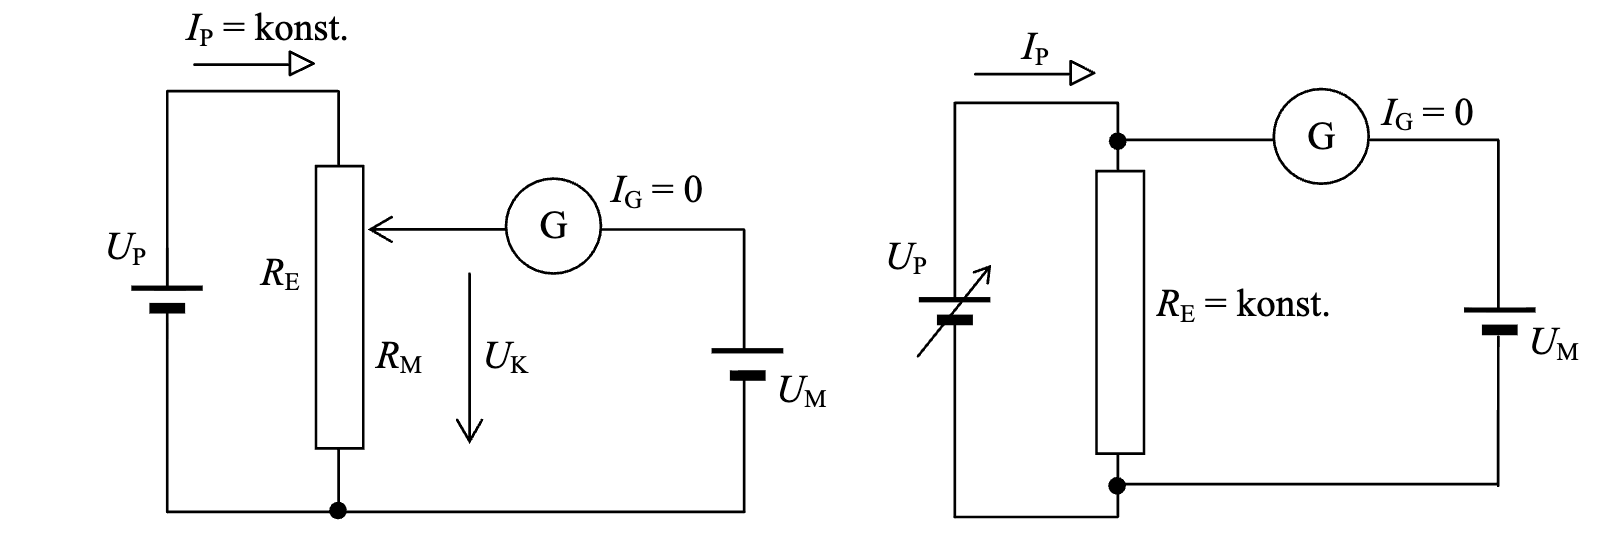
\includegraphics[width=0.70\textwidth]{Obrazky/MVA/kompmetody}
\caption{Kompenzační metoda měření napětí (obr.~7.2a). Pomocný proud $I_0$ je udržován konstantní; odporníkem $R_E$ se nastavuje kompenzační napětí $U_K$ až do rovnováhy s $U_x$.}
\label{fig:kompmetody}
\end{figure}

\textbf{Ampérmetry} se připojují do série. Vnitřní odpor $R_A$ musí být minimální. Zvětšení rozsahu se provádí paralelním bočníkem:
\[ R_B = \frac{R_A}{n-1}, \quad n = \frac{I_{\text{nový}}}{I_{\text{původní}}} \]

\subsection{Výkon v jednofázové střídavé soustavě}
Okamžitý výkon: $p(t) = u(t) \cdot i(t)$. Pro harmonické průběhy platí:
\[ P = U I \cos\varphi \;\text{(činný, W)}, \quad Q = U I \sin\varphi \;\text{(jalový, var)}, \quad S = U I \;\text{(zdánlivý, VA)}, \quad S^2 = P^2 + Q^2 \]
Činný výkon se měří \textbf{wattmetrem}. Wattmetr se zapojuje dvěma způsoby:
\begin{itemize}
    \item \textbf{Zapojení VA} (napěťová cívka přímo na svorkách zátěže): wattmetr změří výkon zátěže navýšený o výkon proudové cívky. Vhodné pro \textbf{velkou} zátěž ($R_Z \gg R_{WI}$).
    \item \textbf{Zapojení AV} (proudová cívka je společná se zátěží i napěťovou cívkou): wattmetr změří výkon navýšený o výkon napěťové cívky. Vhodné pro \textbf{malou} zátěž ($R_Z \ll R_{WU}$).
\end{itemize}
Systematická odchylka obou metod se koriguje odečtením spotřeby příslušné cívky.

\subsection{Měření výkonu v třífázových soustavách -- Aronovo zapojení}
Pro třívodičové soustavy (bez nulového vodiče, symetrické i nesymetrické zátěže) se používají dva wattmetry. Proudové cívky se zapojí do fází $L_1$ a $L_2$, napěťové cívky se připojí k fázi $L_3$:
\[ P = P_1 + P_2 = U_{13} I_1 \cos(\varphi + 30^\circ) + U_{23} I_2 \cos(\varphi - 30^\circ) \]
Při induktivním účiníku $\cos\varphi < 0{,}5$ může jeden z wattmetrů ukazovat zápornou hodnotu.

\begin{figure}[h]
\centering
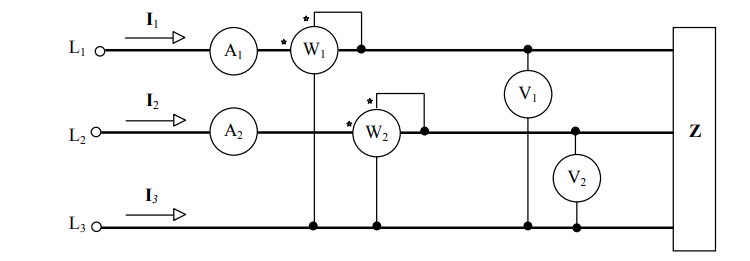
\includegraphics[width=0.80\textwidth]{Obrazky/MVA/aron}
\caption{Aronovo (dvouwattmetrové) zapojení pro třívodičovou soustavu (obr.~7.21). Proudové cívky $W_1$, $W_2$ jsou v sérii s $L_1$, $L_2$; napěťové cívky obou přístrojů se vztahují k fázi $L_3$.}
\label{fig:aron}
\end{figure}

\section{Měření kmitočtu a fázového posuvu}

\subsection{Metody měření kmitočtu}
\begin{itemize}
    \item \textbf{Číslicové čítače (kmitoměry):}
    \begin{itemize}
        \item \textit{Přímé měření:} Čítá se počet period měřeného signálu za přesně definovaný časový interval $T_{gate}$ (např. 1\,s). Absolutní chyba $\pm 1$ perioda. Vhodné pro \textbf{vysoké} kmitočty.
        \item \textit{Měření periody:} Měřený signál otevře hradlo na dobu jedné periody $T_x$, během níž se čítají impulsy referenčního oscilátoru $f_{ref}$ (např. 10\,MHz). Vhodné pro \textbf{nízké} kmitočty (lepší rozlišení).
    \end{itemize}
    \item \textbf{Heterodynní metoda:} Měřený kmitočet $f_x$ se porovnává s nastavitelným referenčním oscilátorem $f_O$. Záznějový signál $\Delta f = |f_x - f_O|$ se při přiblížení $f_O \to f_x$ blíží nule -- stav nulového záznění indikuje rovnost kmitočtů.
    \item \textbf{Rezonanční kmitoměry:} Laditelný LC obvod se nalaďuje do rezonance s měřeným signálem (maximum amplitudy). Používají se pro vyšší kmitočty.
\end{itemize}

\begin{figure}[H]
\centering
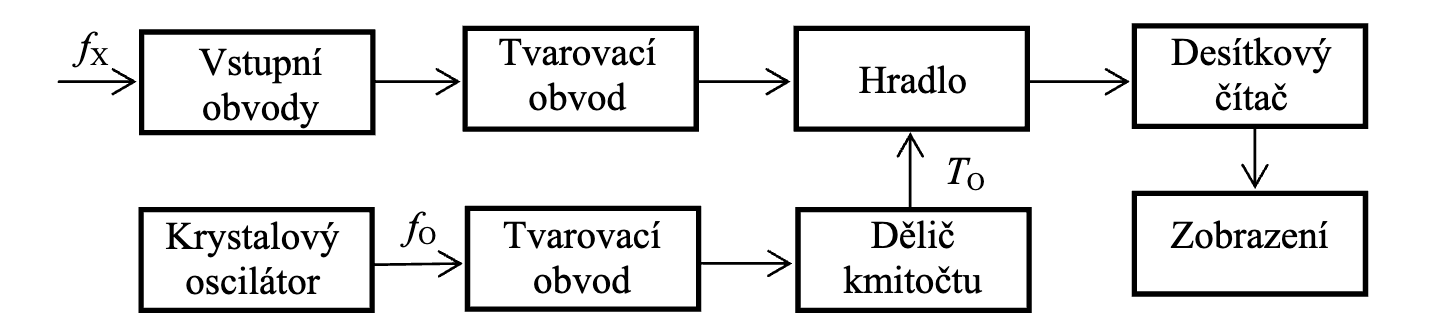
\includegraphics[width=0.72\textwidth]{Obrazky/MVA/citackmitoctu}
\caption{Blokové schéma číslicového čítače -- přímé měření kmitočtu (obr.~7.26). Tvarovač upraví signál na impulsy; hradlo je otevřeno po dobu $T_{gate}$ řízenou krystalovým oscilátorem; čítač zobrazí výsledný kmitočet.}
\label{fig:citac}
\end{figure}

\subsection{Metody měření fázového posuvu}
\begin{itemize}
    \item \textbf{Lissajousovy obrazce:} Dva harmonické signály stejné frekvence se přivedou na vstupy X a Y osciloskopu. Vznikne elipsa. Fázový posun se určí jako $\sin \varphi = A/B$, kde $A$ je průsečík elipsy s osou Y a $B$ je maximální vertikální rozměr elipsy.
    \item \textbf{Časová metoda na osciloskopu:} Změří se časové zpoždění $\Delta t$ mezi průchody nulou obou signálů a perioda $T$:
    \[ \varphi = \frac{\Delta t}{T} \cdot 360^\circ \]
    \item \textbf{Číslicová start-stop metoda:} Tvarovače vytvoří z obou signálů úzké impulsy při průchodu nulou. První impuls (Start) otevře a druhý (Stop) zavře hradlo čítače. Počet napočítaných impulsů reference odpovídá časovému posunu $\Delta t$.
\end{itemize}

\begin{figure}[h]
\centering
\begin{tikzpicture}[>=stealth,scale=1.15]
  \begin{scope}[xshift=0cm]
    \draw[->] (-1.3,0) -- (1.3,0) node[right,font=\scriptsize] {$u_1$};
    \draw[->] (0,-1.3) -- (0,1.3) node[above,font=\scriptsize] {$u_2$};
    \draw[thick,primary] (-1,-1) -- (1,1);
    \node[below,font=\small] at (0,-1.7) {$\varphi = 0^\circ$};
    \node[above right,primary,font=\scriptsize] at (0.5,0.5) {přímka};
  \end{scope}
  \begin{scope}[xshift=3.6cm]
    \draw[->] (-1.3,0) -- (1.3,0) node[right,font=\scriptsize] {$u_1$};
    \draw[->] (0,-1.3) -- (0,1.3) node[above,font=\scriptsize] {$u_2$};
    \draw[thick,primary,smooth,domain=0:360,samples=60]
      plot ({sin(\x)},{sin(\x+45)});
    \filldraw[accent] (0,{sin(45)}) circle (1.6pt);
    \node[right,accent,font=\scriptsize] at (0.05,{sin(45)}) {$A$};
    \draw[dashed,gray] (-1.15,1) -- (1.15,1);
    \draw[<->,accent!80!black] (1.1,0) -- (1.1,1) node[midway,right,font=\scriptsize] {$B$};
    \node[below,font=\small] at (0,-1.7) {$\varphi = 45^\circ$};
  \end{scope}
  \begin{scope}[xshift=7.2cm]
    \draw[->] (-1.3,0) -- (1.3,0) node[right,font=\scriptsize] {$u_1$};
    \draw[->] (0,-1.3) -- (0,1.3) node[above,font=\scriptsize] {$u_2$};
    \draw[thick,primary,smooth,domain=0:360,samples=60]
      plot ({sin(\x)},{cos(\x)});
    \filldraw[accent] (0,1) circle (1.6pt) node[right,font=\scriptsize] {$A{=}B$};
    \node[below,font=\small] at (0,-1.7) {$\varphi = 90^\circ$};
  \end{scope}
\end{tikzpicture}
\caption{Lissajousovy obrazce pro různé fázové posuny (stejná frekvence). $A$ = průsečík elipsy s osou $u_2$, $B$ = amplituda $u_2$. Fázový posun: $\sin\varphi = A/B$.}
\label{fig:lissajous}
\end{figure}


\chapter{Měření pasivních elektrických veličin}
\label{ch:pasivni_veliciny}

\noindent\textit{Ohmova (voltampérová) metoda měření odporu (vliv vnitřních odporů přístrojů), stejnosměrné můstky (Wheatstoneův, Thomsonův), ohmmetry, střídavé můstky (Maxwell-Wienův, Scheringův), rezonanční metoda (Q-metr), číslicové a vektorové metody měření impedancí (auto-balancing bridge, I-V metoda), neelektrické snímače využívající pasivní prvky (Pt100, tenzometry, kapacitní a indukční snímače).}

\section{Měření stejnosměrného odporu}

\subsection{Voltampérová (Ohmova) metoda}
Odpor se určí z naměřeného napětí a proudu ($R = U/I$). Podle zapojení vzniká systematická chyba metody způsobená spotřebou měřicích přístrojů:

\begin{itemize}
    \item \textbf{Zapojení pro malé odpory (měření napětí přímo na $R_x$):}
          Proud protékající ampérmetrem se dělí do měřeného odporu $R_x$ a do voltmetru s vnitřním odporem $R_V$. Naměřená hodnota odporu je zatížena chybou:
          \[ R_{\text{nam}} = \frac{U}{I} = \frac{R_x \cdot R_V}{R_x + R_V} < R_x \]
          Metoda je vhodná pro $R_x \ll R_V$, kdy proud voltmetrem je zanedbatelný.
    \item \textbf{Zapojení pro velké odpory (měření proudu přímo přes $R_x$):}
          Voltmetr měří napětí na odporu $R_x$ navýšené o úbytek na vnitřním odporu ampérmetru $R_A$. Naměřená hodnota je:
          \[ R_{\text{nam}} = \frac{U}{I} = R_x + R_A > R_x \]
          Metoda je vhodná pro $R_x \gg R_A$, kdy úbytek napětí na ampérmetru je zanedbatelný.
\end{itemize}

\subsection{Stejnosměrné můstky}
Můstky slouží k přesnému srovnávacímu měření odporů.

\subsubsection{Wheatstoneův můstek}
Používá se pro střední odpory ($1\ \Omega$ až $1\text{ M}\Omega$).

\begin{figure}[h]
\centering
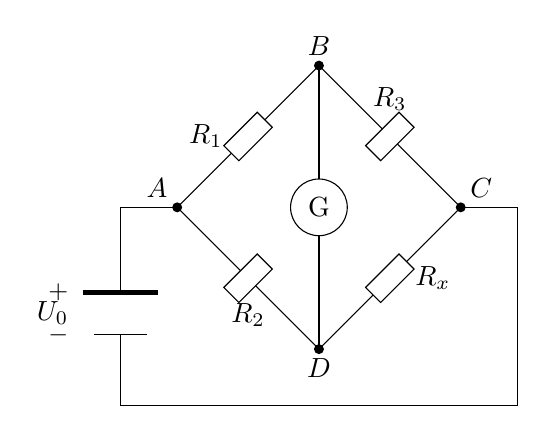
\begin{tikzpicture}[scale=1.2]
  \coordinate (A) at (0,0);
  \coordinate (B) at (1.5,1.5);
  \coordinate (C) at (3,0);
  \coordinate (D) at (1.5,-1.5);

  \draw (A) -- (B) node[midway, draw, fill=white, rotate=45,  minimum width=0.6cm, minimum height=0.27cm, label={135:$R_1$}] {};
  \draw (B) -- (C) node[midway, draw, fill=white, rotate=45, minimum width=0.6cm, minimum height=0.27cm, label={45:$R_3$}] {};
  \draw (A) -- (D) node[midway, draw, fill=white, rotate=45, minimum width=0.6cm, minimum height=0.27cm, label={225:$R_2$}] {};
  \draw (D) -- (C) node[midway, draw, fill=white, rotate=45,  minimum width=0.6cm, minimum height=0.27cm, label={315:$R_x$}] {};

  \draw (B) -- (D);
  \draw[fill=white] (1.5,0) circle (0.3) node {G};

  \fill (A) circle (1.5pt) node[above left]  {$A$};
  \fill (B) circle (1.5pt) node[above] {$B$};
  \fill (C) circle (1.5pt) node[above right] {$C$};
  \fill (D) circle (1.5pt) node[below] {$D$};

  \draw (A) -- (-0.6,0) -- (-0.6,-0.9);
  \draw (-0.6,-1.35) -- (-0.6,-2.1) -- (3.6,-2.1) -- (3.6,0) -- (C);
  \draw[line width=2pt] (-1.0,-0.9)  -- (-0.2,-0.9);
  \draw                 (-0.88,-1.35) -- (-0.32,-1.35);
  \node[left, font=\small] at (-1.05,-0.9)  {$+$};
  \node[left, font=\small] at (-1.05,-1.35) {$-$};
  \node[left] at (-1.05,-1.12) {$U_0$};
\end{tikzpicture}
\caption{Schéma vyváženého Wheatstoneova můstku}
\label{fig:wheatstone}
\end{figure}

Při nulovém proudu galvanometrem ($I_G = 0$) je můstek vyvážen a platí:
\[ R_x = R_2 \frac{R_3}{R_1} \]
U nevyváženého můstku je výstupní napětí $U_{BD}$ úměrné malé změně měřeného odporu $\Delta R_x$, což se využívá např. u tenzometrických snímačů.

\subsubsection{Thomsonův (dvojitý) můstek}
Používá se pro měření velmi malých odporů (pod $1\ \Omega$, např. vinutí, kontaktní odpory). Problém Wheatstoneova můstku -- vliv odporu přívodních vodičů $r$ -- řeší \textbf{čtyřsvorkové (Kelvinovo) zapojení} měřeného odporu $R_x$ a etalonu $R_N$. Podmínka rovnováhy:
\[ R_x = R_N \cdot \frac{R_1}{R_2}, \qquad \text{podmínka eliminace vlivu } r\text{: } \frac{r_1}{r_2} = \frac{R_1}{R_2} \]
Jsou-li poměry splněny, vliv $r$ se zcela vyruší a výsledek nezávisí na odporu spojení.

\subsection{Ohmmetry}
Ohmmetr měří odpor přímo -- obsahuje vlastní zdroj napájení (baterie) a měřicí přístroj (magnetoelektrické ústrojí).

\begin{itemize}
    \item \textbf{Sériový ohmmetr:} Zdroj $U$, regulační odpor $R_0$ (justáž nuly) a přístroj $R_M$ jsou zapojeny sériově; $R_x$ se připojí do série.
    \[ I = \frac{U}{R_0 + R_M + R_x} \]
    Při $R_x = 0$: plná výchylka ($0\ \Omega$, vpravo). Při $R_x \to \infty$: nulová výchylka ($\infty$, vlevo). Stupnice je nelineární. Vhodný pro střední odpory. Před každým měřením nutná \textit{justáž nuly}.
    \item \textbf{Paralelní ohmmetr:} $R_x$ je zapojen paralelně s přístrojem. Při $R_x = 0$: nulová výchylka ($0\ \Omega$, vlevo). Při $R_x \to \infty$: plná výchylka (vpravo). Vhodný pro malé odpory (pod $100\ \Omega$).
\end{itemize}

\section{Měření střídavé impedance}
Impedance $\mathbf{Z} = R + jX$ má dvě složky (reálnou a reaktivní), proto střídavé měřicí obvody vyžadují vyvážení ve dvou parametrech (amplituda i fáze).

\subsection{Střídavé můstky}
Napájeny jsou AC generátorem, jako indikátor rovnováhy slouží selektivní detektor. Obecná podmínka rovnováhy střídavého můstku: $\mathbf{Z}_x \mathbf{Z}_1 = \mathbf{Z}_2 \mathbf{Z}_3$.
\begin{itemize}
    \item \textbf{Maxwell-Wienův můstek:} Porovnává indukčnost ($L_x, R_x$) s kapacitním standardem ($C_4, R_4$) v protilehlé větvi. Vyvažovací podmínky jsou nezávislé na frekvenci:
          \[ L_x = R_2 R_3 C_4, \quad R_x = \frac{R_2 R_3}{R_4} \]

\begin{figure}[h]
\centering
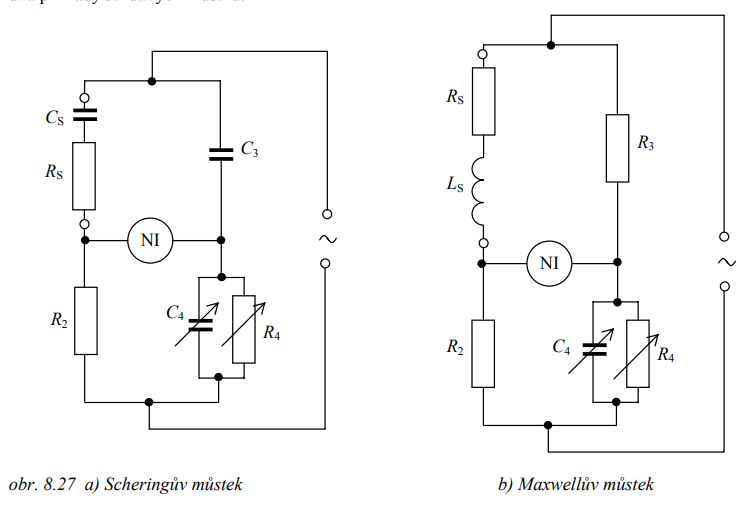
\includegraphics[width=0.45\textwidth]{Obrazky/MVA/maxwell}
\caption{Maxwellův můstek (obr.~8.27b): neznámá indukčnost $L_s$ s~odporem $R_s$ se porovnává s~kapacitním standardem $C_4 \parallel R_4$. Podmínky rovnováhy nezávislé na kmitočtu: $L_s = C_4 R_2 R_3$, $R_s = R_2 R_3 / R_4$.}
\label{fig:maxwell_wien}
\end{figure}

    \item \textbf{Scheringův můstek:} Používá se pro měření kapacity $C_x$ a ztrátového činitele $\tan\delta$ (kondenzátory, izolace) při vysokých napětích. Podmínky rovnováhy:
          \[ C_x = C_N \frac{R_2}{R_3}, \qquad \tan\delta_x = \omega R_2 C_2 \]
          Výhodou je, že $\tan\delta$ závisí pouze na nízkonapěťových součástkách $R_2$, $C_2$.
\end{itemize}

\subsection{Rezonanční metoda (Q-metr)}
Využívá vlastností sériového rezonančního obvodu tvořeného neznámou cívkou ($L_x, R_x$) a přesným ladicím kondenzátorem $C$.
Při rezonanci ($\omega L_x = 1/(\omega C)$) napětí na kondenzátoru $U_C$ vzroste vůči vstupnímu napětí $U_i$ podle činitele jakosti cívky $Q$:
\[ Q = \frac{\omega L_x}{R_x} = \frac{U_C}{U_i} \]
Z naměřeného $U_C$, kmitočtu $\omega$ a kapacity $C$ při rezonanci se dopočítají parametry cívky: $L_x = 1/(\omega^2 C)$ a $R_x = \omega L_x / Q$.

\subsection{Číslicové a vektorové metody měření impedancí}
Moderní automatické LCR metry pracují na principu:
\begin{itemize}
    \item \textbf{Vektorová I-V metoda:} Měří se komplexní napětí na součástce $\mathbf{U}_x$ a komplexní proud $\mathbf{I}_x$ (jako úbytek napětí na známém referenčním rezistoru). Fázově citlivé detektory určí reálnou a imaginární složku, z nichž se spočítá $\mathbf{Z}_x = \mathbf{U}_x/\mathbf{I}_x$.
    \item \textbf{Metoda s automaticky vyvažovaným můstkem (Auto-balancing bridge):} Proud protékající součástkou $\mathbf{Z}_x$ je odváděn virtuální nultou zemí operačního zesilovače do referenčního rezistoru $R_r$. Napětí na výstupu OZ odpovídá proudu $\mathbf{I}_x$. Velmi přesné v širokém frekvenčním rozsahu (do 100 MHz).
\end{itemize}

\section{Snímače neelektrických veličin využívající pasivní prvky}
Převádějí neelektrickou veličinu (teplota, poloha, deformace) na změnu elektrického odporu, kapacity či indukčnosti.

\begin{itemize}
    \item \textbf{Odporové snímače teploty (RTD):}
          \begin{itemize}
              \item \textbf{Pt100:} Platinový snímač (odpor $100\ \Omega$ při $0^\circ\text{C}$). Kladný teplotní součinitel (PTC), vysoká linearita a stabilita.
              \item \textbf{Termistory:} Polovodičové snímače. NTC (odpor s teplotou exponenciálně klesá, vysoká citlivost) nebo PTC (odpor v určitém bodě prudce vzroste). Značná nelinearita.
              \item \textbf{Termočlánky:} Využívají Seebeckův jev -- napětí vznikající na spoji dvou různých kovů při rozdílu teplot: $U = \alpha (T_{\text{měř}} - T_{\text{srov}})$
          \end{itemize}
    \item \textbf{Tenzometrické snímače (síla, tlak):} Kovové fólie nalepené na pružném tělese. Při deformaci $\Delta l/l$ dochází ke změně odporu:
          \[ \frac{\Delta R}{R} = G \cdot \frac{\Delta l}{l} \]
          kde $G$ je deformační činitel ($G \approx 2$ u kovů, $G \approx 100$ u polovodičů). Zapojují se do Wheatstoneova můstku kvůli teplotní kompenzaci.
    \item \textbf{Kapacitní snímače (poloha, posuv):} Využívají změnu kapacity deskového kondenzátoru $C = \varepsilon \frac{S}{d}$. Změnou vzdálenosti desek $d$ (nelineární), změnou plochy překryvu $S$ (lineární) nebo změnou permitivity dielektrika $\varepsilon$ (měření hladiny, vlhkosti).
    \item \textbf{Indukční snímače (poloha, posuv):} Využívají změnu indukčnosti cívky změnou vzduchové mezery v magnetickém obvodu. Často se používají v diferenciálním zapojení jako lineární diferenciální transformátor (LVDT) pro vysoce přesné měření polohy.
\end{itemize}

\begin{figure}[h]
\centering
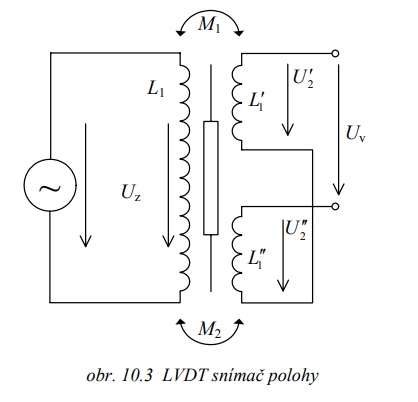
\includegraphics[width=0.55\textwidth]{Obrazky/MVA/lvdt}
\caption{Lineární diferenciální transformátor -- LVDT (obr.~10.3). Primár napájený střídavým napětím indukuje v obou sekundárech. Pohybem feromagnetického jádra se mění magnetická vazba: $U_2'$ roste, $U_2''$ klesá. Diferenciální výstup $U_v = U_2' - U_2''$ je lineárně úměrný posuvu $x$, ve středové poloze je $U_v = 0$.}
\label{fig:lvdt}
\end{figure}
